\begin{figure}[htbp]
    \centering
    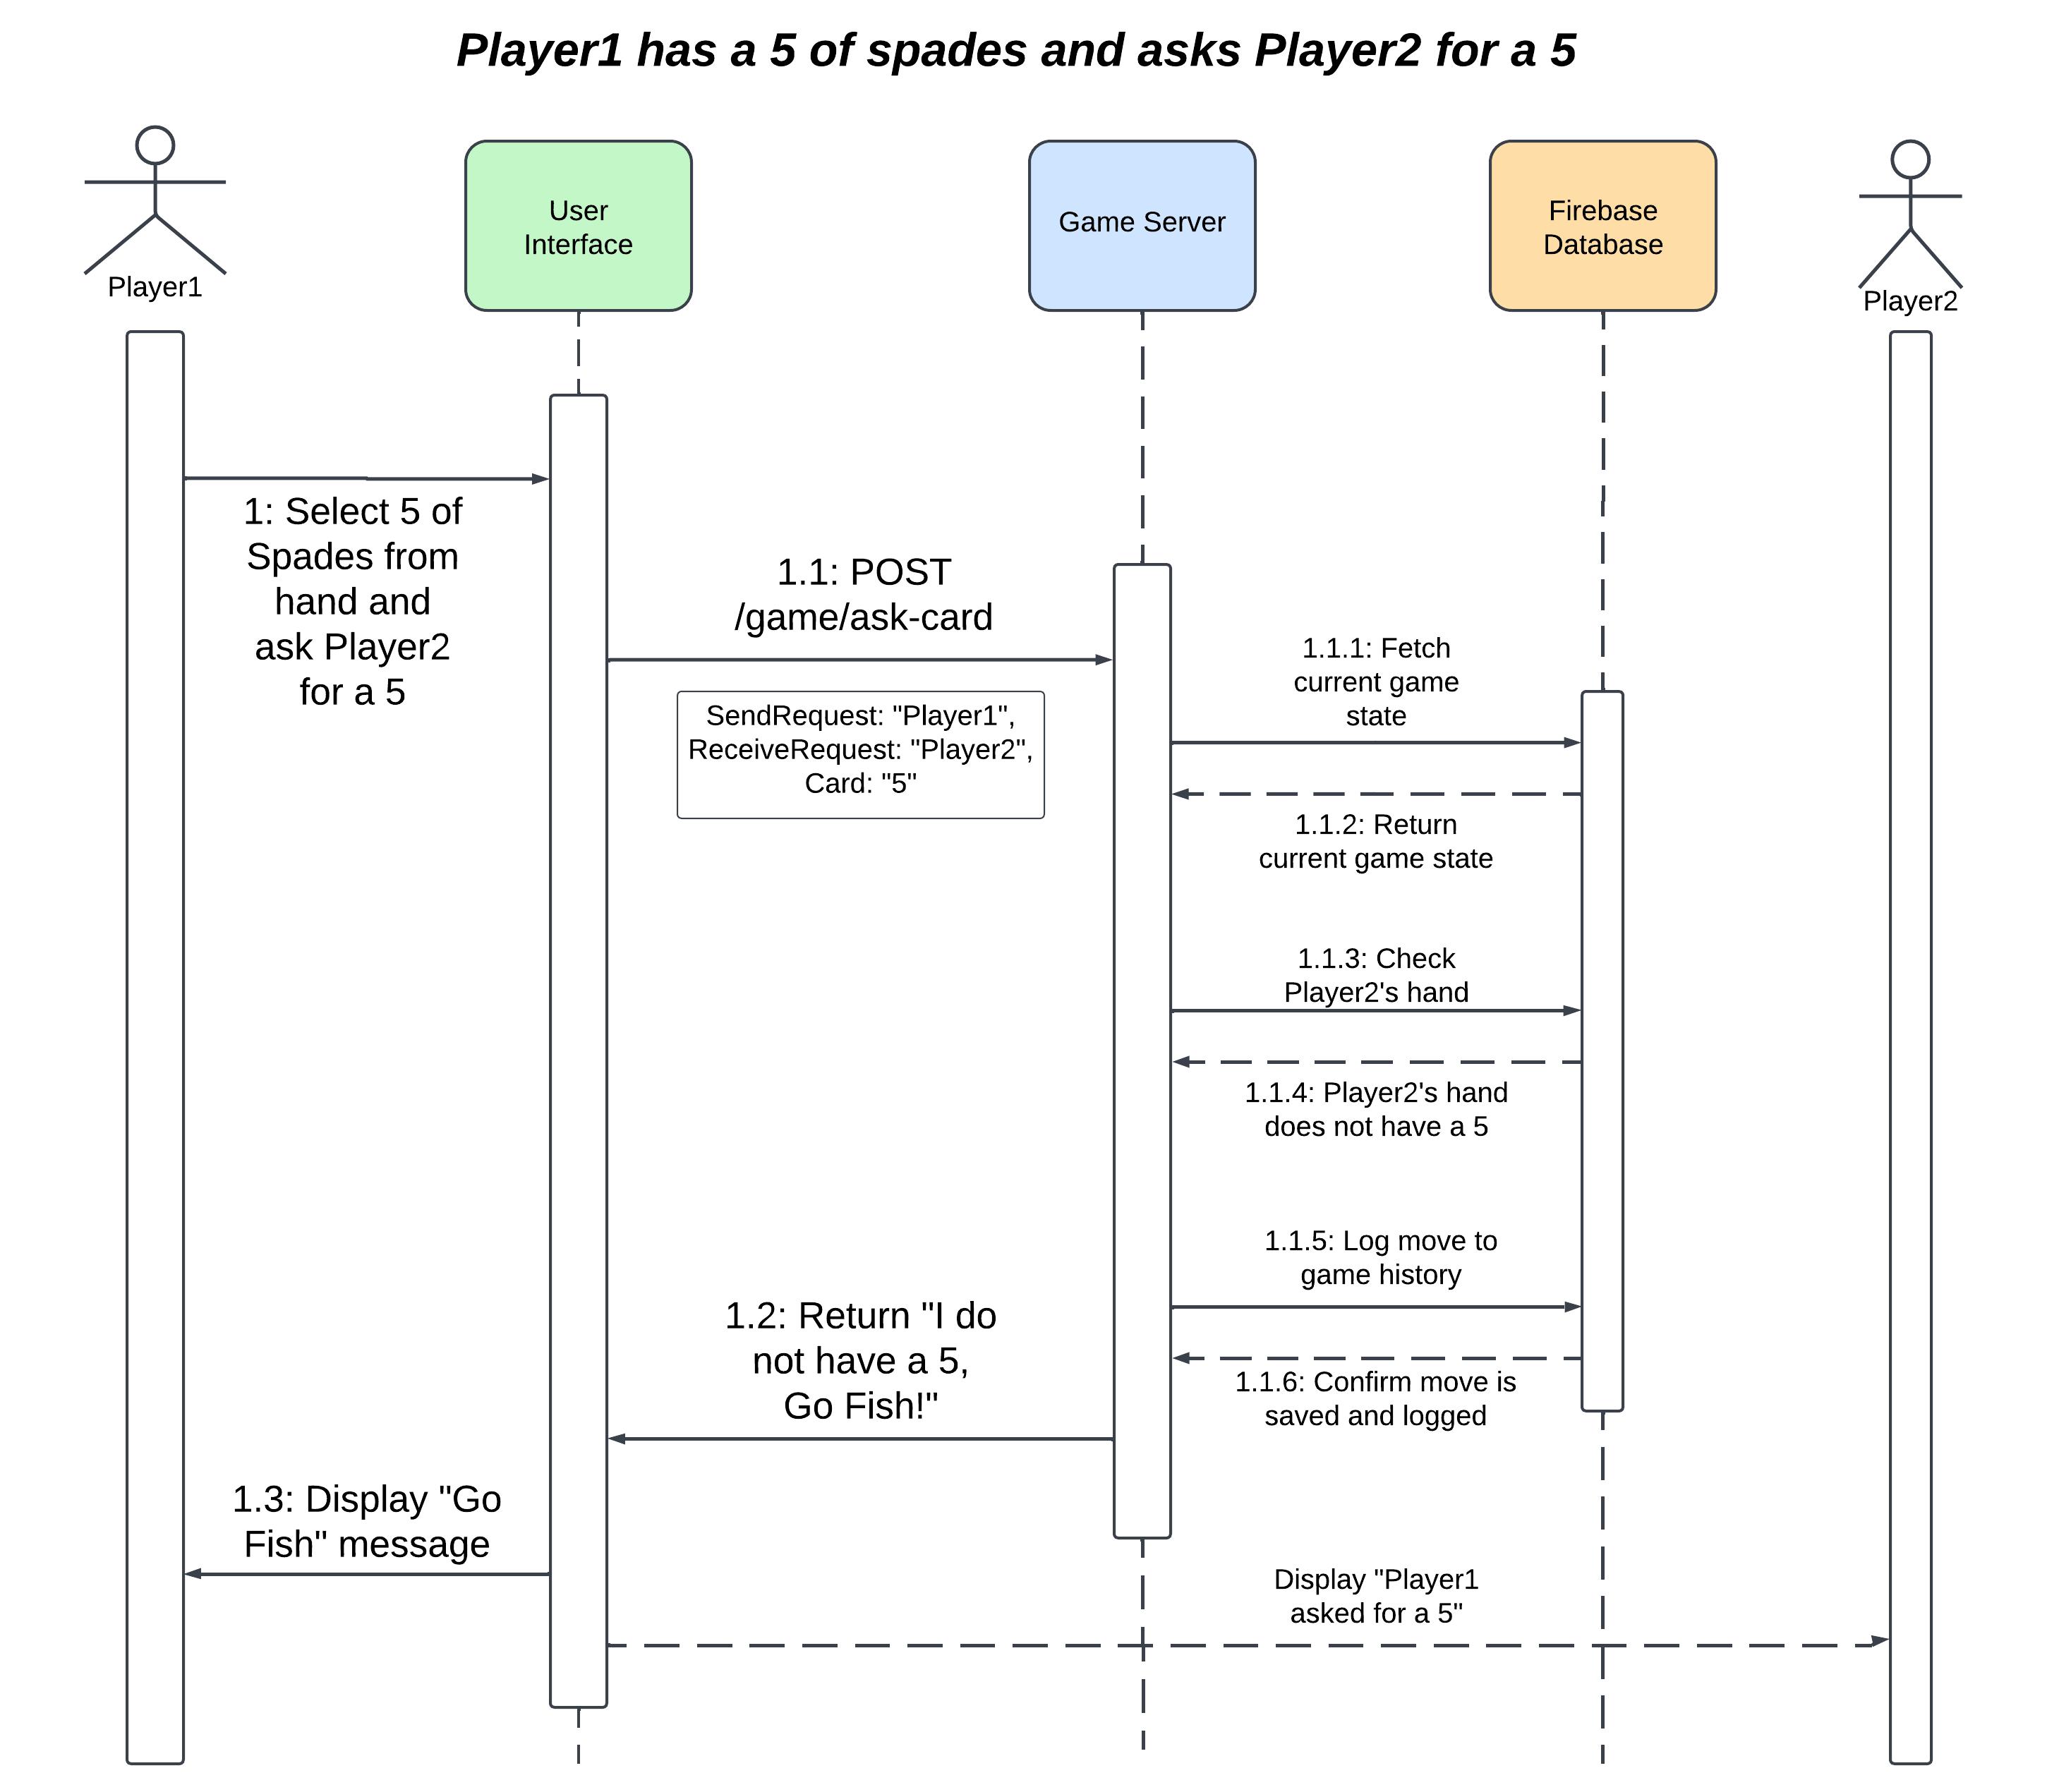
\includegraphics[width=1\linewidth]{CS482 Sequence Diagram Sprint 2.png}
    \caption{UML sequence diagram of Player1 asking Player2 for a card they do not have, resulting in Player1 being told to "Go Fish"}
    \label{fig:umlsequence}
\end{figure}

This UML sequence diagram illustrates the process of a player asking for a specific card during gameplay. In this scenario, Player1 selects a 5 of Spades from their hand and asks Player2 if they have any cards of the same rank. Player2, however, does not possess a 5, leading to the "Go Fish!" outcome for Player1.

The sequence begins with Player1 selecting the card and initiating a request through the game's user interface. This request is sent to the game server, which forwards it to the database to fetch Player2's current hand. The database responds with the data, enabling the server to check if Player2 has a 5. Upon finding that Player2 does not have the requested card, the server logs the move, saves the interaction in the game history, and returns a response to the user interface indicating that Player1 must "Go Fish!" The user interface then displays this message, completing the sequence.

\begin{figure}[htbp]
    \centering
    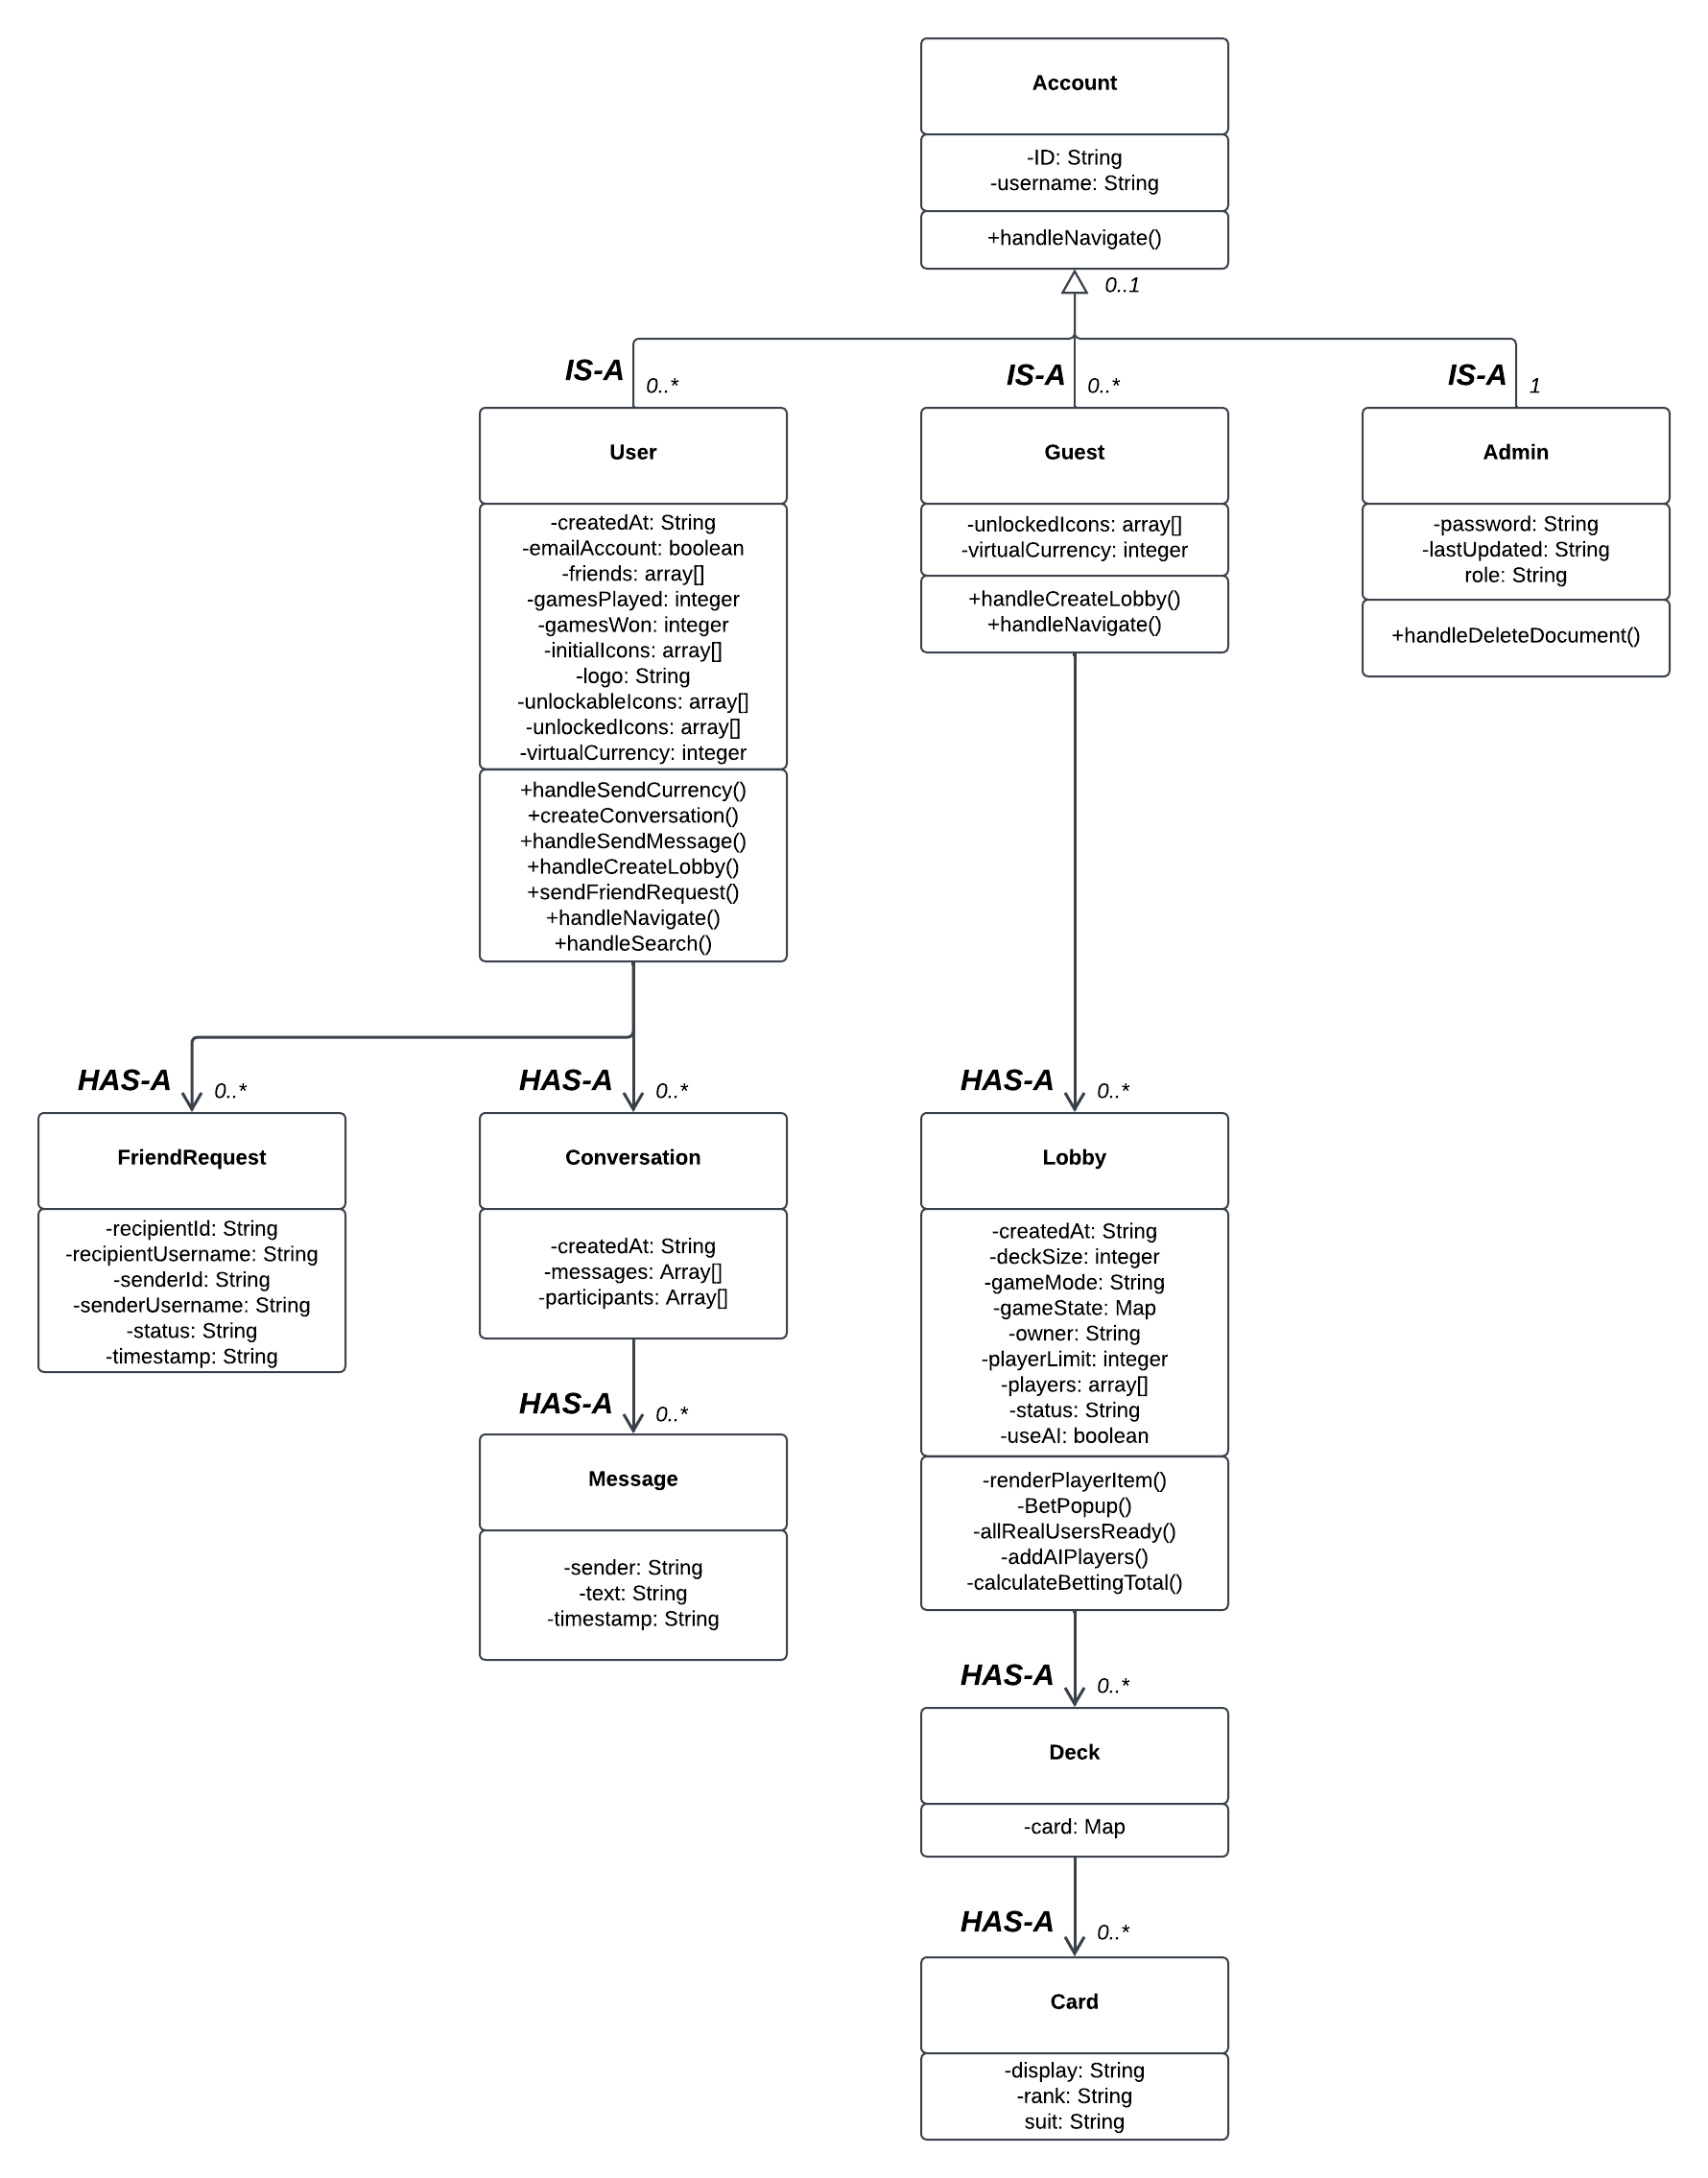
\includegraphics[width=1\linewidth]{CS482 Sequence Diagram Sprint 3.png}
    \caption{UML class diagram showing the system's structure, including key entities, their attributes, methods, and relationships.}
    \label{fig:umlclass}
\end{figure}

This UML class diagram provides an overview of the system’s architecture, detailing the primary classes, their attributes, methods, and relationships. At the top of the hierarchy is the `Account` class, which serves as a base class with attributes such as `ID` and `username` and a method to handle navigation. Three subclasses inherit from `Account`: `User`, `Guest`, and `Admin`, each with their specific attributes and methods. 

The `User` class has attributes like `friends`, `gamesPlayed`, `gamesWon`, and `virtualCurrency`, along with methods for sending currency, creating conversations, and handling lobbies. The `Guest` class is a simplified version of the `User`, with attributes and methods limited to navigation and lobby creation. Meanwhile, the `Admin` class includes additional capabilities for moderation, such as handling document deletion and role management.

Several associated entities represent the system’s functionality:
- The `FriendRequest` class represents friend requests with attributes such as sender/recipient details and status.
- The `Conversation` class manages messaging with participants and a collection of `Message` instances, each containing details like sender, text, and timestamp.
- The `Lobby` class includes attributes like `gameMode`, `gameState`, and `players`, along with methods for managing players, calculating bets, and handling AI.
- The `Deck` and `Card` classes manage the game’s deck and cards, respectively, with attributes for ranks, suits, and display information.

The diagram captures key `IS-A` (inheritance) and `HAS-A` (composition/aggregation) relationships, illustrating how the components interact to support the system’s functionality. It emphasizes modularity and scalability, ensuring the system can accommodate future expansions or changes.
